The dataset \cite{brain-dataset} contained 5000 JPG-format head CT images from 82 patients, evenly split between 2500 brain window images and 2500 bone window images. Each patient had about 30 slices. Intracranial hemorrhage masks were available for 318 images, though not required for classification. Two CSV files provided hemorrhage diagnosis data and patient demographic/clinical data.

For this study, only binary classification was relevant: cases were classified as positive (any hemorrhage present) or negative (no hemorrhage). Exploratory analysis revealed 36 patients with hemorrhage and 46 without. Only brain window images were analyzed.

\begin{figure}[htbp]
    \centerline{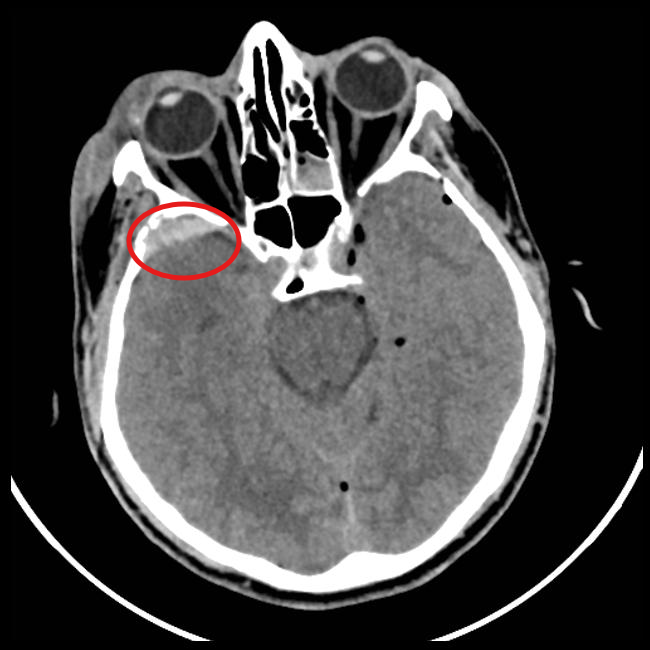
\includegraphics[width=0.45\linewidth]{imgs//dataset/positive.png}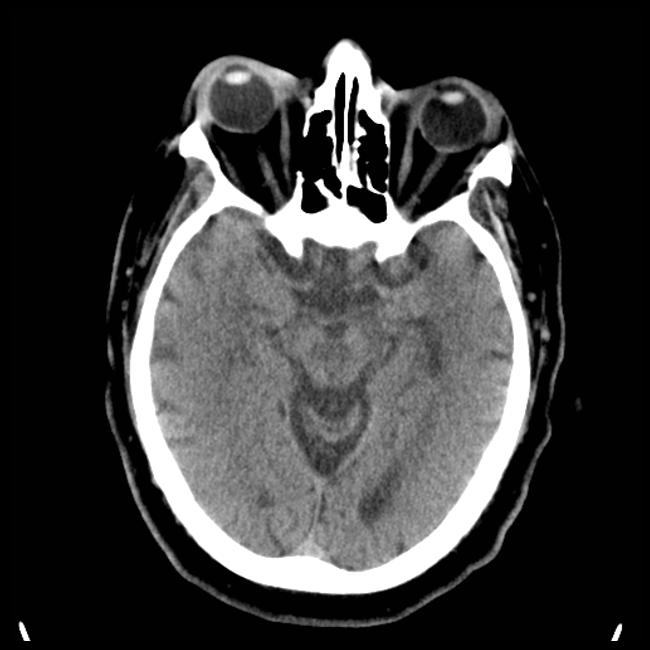
\includegraphics[width=0.45\linewidth]{imgs//dataset/negative.png}}
    \caption{Brain with hemorrhage vs brain without hemorrhage.}
    \label{fig:brain_images}
\end{figure}

Since masks are not needed for classification, nor the bone images, we removed the mask images (which contained \quotes{HSE\_Seg} in their name). Similarly, the whole bone folder was removed for each patient. Finally, we moved and separated patients into two folders, depending on whether they were positive or negative cases.

\begin{figure}[h]
    \centering
    \scalebox{0.5}{\begin{tikzpicture}[>=latex,shorten >=2pt,shorten <=2pt,shape aspect=1]
    % Define the rectangle nodes
    \node (Masks) [rectangle, draw, minimum height=1.8cm, minimum width=3cm, text width=2.5cm, align=center] {Remove mask images};
    
    \node (Bones) [rectangle, draw, minimum height=1.8cm, minimum width=3cm, text width=2.5cm, align=center] at ([xshift=3cm]Masks.east) {Remove bone images};
    
    \node (Inclusion) [rectangle, draw, minimum height=1.8cm, minimum width=3cm, text width=2.5cm, align=center] at ([xshift=3cm]Bones.east) {Move patients to positive or negative directories};

    % Draw arrows between the nodes
    \draw[->, thick] (Masks.east) -- (Bones.west);
    \draw[->, thick] (Bones.east) -- (Inclusion.west);
\end{tikzpicture}
}
    \caption{Preprocessing flow.}
    \label{fig:preprocessing_flow}
\end{figure}
